%! Author = Len Washington III
%! Date = 10/14/24

% Preamble
\documentclass[
	chapter=6,
	title={Thermochemistry},
	showanswers=true,
]{chem122notes}

% Packages

% Document
\begin{document}

Chapters 1-5 study matter, now we study energy.

Warming your hands with chemical hand warmers involves many of the principles of \emph{thermochemistry}, the study of the relationships between chemistry and energy.
When you open the package that contains the hand warmer, the contents are exposed to air, and a reaction that gives off heat to its surroundings occurs.
Most handwarmers\label{dfn:chemical-handwarmers} involve the oxidation of iron:
\[ \ce{4Fe(s) + 3O2(g) -> 2Fe2O3(s)} \]

In this chapter, we look at how chemical reactions can exchange energy with their surroundings and how we can quantify the magnitude of those exchanges.

\subsection{Applications}\label{subsec:applications}
\begin{itemize}
	\item Heating of homes
	\item Production of energy
\end{itemize}

\section{Key Definitions}\label{sec:key-definitions}
\begin{description}
	\item[Energy] Capacity to do work
	\item[Work] Result of a force active through a distance
	\item[Examples of work]~
	\begin{itemize}
		\item Pushing a box across the floor
		\item a billiard ball rolling across a billiard table and colliding with a second, stationary ball
	\end{itemize}
	\item[Potential energy] Associated with position or composition. Example: Raising a billiard ball off the table increases its potential energy.
	\item[Chemical energy] Associated with relative positions of electrons and nuclei in atoms and molecules
	% TODO: Add Tikz representation of tree
	\item[Law of conservation of energy] energy can be neither created nor destroyed; it can assume different forms
	\item[System] chemicals in a beaker (or handwarmers) for example
	\item[Surrounding] water that the chemicals are dissolved in, the beaker, the lab bench, air in the room, etc.
	\begin{itemize}
		\item Surroundings gain the exact amount of energy lost by the system and vice versa.
	\end{itemize}
\end{description}

\section{Units of Energy}\label{sec:units-of-energy}
\begin{itemize}
	\item $KE = \frac{1}{2}mv^{2}$, $[KE] = [m][v] = \mbox{kg}\times \frac{m}{s}$
	\item 1 Joule (J) = $1\ \frac{\mbox{kg } \mbox{m}^{2}}{\mbox{s}^{2}}$
	\item 1 calorie = 4.184 J
\end{itemize}

\section{1st law of thermodynamics}\label{sec:sec:1st-law-of-thermodynamics}
\begin{itemize}
	\item The total energy of the universe is constant $\rightarrow$ Energy is neither created, nor destroyed, universe does not exchange energy with anything else.
	\item According to the 1st law, a device that continually produces energy with no energy input cannot exist.
\end{itemize}

\subsection{Internal Energy (IE)}\label{subsec:internal-energy-(ie)}
\begin{itemize}
	\item The internal energy of a system is the sum of the kinetic and potential energies of all the particles that compose the systems.
	\item It is a ``state function''.
	\item State of a chemical system is specified by parameters such as temperature, pressure, concentration, and phase (solid, liquid, or gas)
	\item Elevation of 10,000 ft, for example, is a state function no matter how you climbed it;
	the distance, however, is not a state function as you can take any route.
\end{itemize}

\begin{equation*}
\begin{aligned}
	\Delta E &= E_{final} - E_{initial}\\
	\ce{C(s)} + \ce{O2(g)} &\ce{->} \ce{CO2(g)}\\
	\Delta E &= E_{product} - E_{reactant}\\
\end{aligned}
\end{equation*}

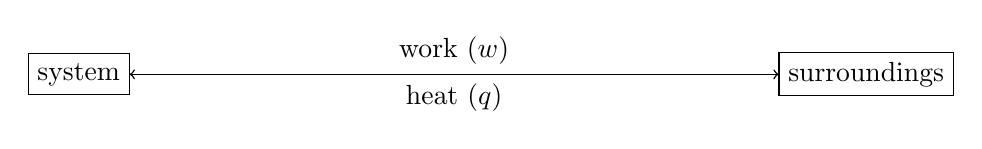
\begin{tikzpicture}
	\begin{scope}\tikzset{every node/.style={rectangle,draw}}
	\node (sys) at (0, 0) {system};
	\node (surr) at (10,0 ) {surroundings};
		%		\node (q) at (5, 2) {};
		%		\node (w) at (5, -2) {};
	\end{scope}
	\begin{scope}
		\path [<->,below,yshift=5] (sys) edge node{heat ($q$)} (surr);
		\path [<->,above,yshift=-5] (surr) edge node{work ($w$)} (sys);
	\end{scope}
\end{tikzpicture}

\begin{itemize}
	\item System can exchange energy with its surrounding through heat and work.
	\item According to 1st law of thermodynamics
\end{itemize}
\begin{equation}
	\Delta E = q + w
	\label{eq:thermodynamics-first-law}
\end{equation}

\section{Quantifying Heat and Work}\label{sec:quantifying-heat-and-work}
Experimentally, $q\propto \Delta t$ where $q$ is heat absorbed by the system and $\Delta t$ is the change of temperature.
\begin{equation}
	q = c \times \Delta t
	\label{eq:heat-capacity}
\end{equation}
where $c$ is the heat capacity (quantity of heat required to change temperature by 1\textdegree{}C).

\begin{equation}
	\begin{aligned}
		q &= m \times s \times \Delta t\\
		[J] &= [g] \times \left[ \frac{J}{g\textdegree C} \right] \times [\textdegree C]
	\end{aligned}
	\label{eq:heat-mass}
\end{equation}
where $m$ is the mass and $s$ is the specific heat.

%\begin{table}[H]
%	\centering
%	\caption{Specific Heat Capcaity Table}
%	\label{tab:specific-heat}
%	\begin{tabular}{|c|c|}
%		\textbf{Substance} & \textbf{Specific Heat Capacity at 25\textdegree{}C in J/g\textdegree{}C}\\
%		{H2} gas & 14.267\\
%		{He} gas & 5.300\\
%		{H2O(l)} & 4.184\\
%	\end{tabular}
%\end{table}

\section{Work: Pressure Volume Work}\label{sec:work:-pressure-volume-work}
\begin{equation}
	\begin{aligned}
		W &= -P\Delta V\\
		  &= -P(V_{f} - V_{i})\\
		  &= P(V_{i} - V_{f})\\
	\end{aligned}
	\label{eq:pressue-volume-work}
\end{equation}
Combustion of gasoline causes gases within the cylinders of an automobile engine to expand, pushing the piston outward and moving the car wheels.

\section{Enthalpy}\label{sec:enthalpy}
\definition{Enthalpy}{Heat evolved in a chemical reaction at constant pressure.}

Firstly, at constant volume (chemical rxn [reaction] in a sealed container):
\begin{equation*}
\begin{aligned}
	W &= -P\Delta V\\
	  &= 0\\
	\Delta E_{rxn} &= q_{v} + w\\
						 &= q_{v}
\end{aligned}
\end{equation*}
When chemical reactions occur open to the atmosphere at constant pressure, both $q$ and $w$ are involved in $\Delta E_{rxn}$.

We are often interested only in $q$, not $w$.
For example, when we burn natural gas in the furnace to heat our homes.

Enthalpy $H$, a new thermodynamic quantity, is thus introduced.
\begin{equation}
	\begin{aligned}
		H &= E + PV\\
		\Delta H &= \Delta E + P\Delta V \ \ \ (\mbox{at constant pressure})\\
		&= (q_{p} + W) + P\Delta V\\
		&= q_{p} + W - W\\
		&= q_{p}
	\end{aligned}
	\label{eq:enthalpy}
\end{equation}

\section{$\Delta E$ and $\Delta H$}\label{sec:e-and-h}
\begin{itemize}
	\item Conceptually they are similar
	\item $\Delta E$ is a measure of all of the energy ($q$ and $w$) exchanged with the surroundings
	\item $\Delta H$ is only a measure of heat exchanged ($q$) under conditions of constant pressure.
	\item For chemical rxns that do not exchange much work with the surroundings, i.e., $W=-P\Delta V$ is small as $\Delta V$ is small, $\Delta H \approx \Delta E$ (nearly identical)
	\item For chemical reactions that produce or consume large amounts of gas, hence have large $\Delta V$ (and hence large $W$), $\Delta H \neq \Delta E$ (significantly different)
\end{itemize}

\section{Exothermic and Endothermic Reactions}\label{sec:exothermic-and-endothermic-reactions}
\begin{itemize}
	\item $\Delta H > 0$ is an endothermic reaction, chemical reaction \emph{absorbs} heat from the surroundings.
	\begin{itemize}
		\item Example: The reaction that occurs in the chemical cold packs used to ice athletic injuries $\rightarrow$ The surroundings, including the bruised wrist, get colder as the cold pack absorbs energy.
	\end{itemize}
	\item $\Delta H < 0$ is an exothermic reaction, chemical reaction \emph{radiates} heat to its surroundings.
	\begin{itemize}
		\item Example: \hyperref[dfn:chemical-handwarmers]{Chemical handwarmers}.
	\end{itemize}
\end{itemize}

\section{Stoichiometry involving $\Delta H$: Thermochemical Equations}\label{sec:stoichiometry-involving-$delta-h$:-thermochemical-equations}
\centerce{C3H8(g) + 5O2(g) -> 3CO2(g) + 4H2O(g)}
\begin{equation*}
\begin{aligned}
	\Delta H_{rxn} &= -2044 kJ\\
	1 \mbox{ mol } \ce{C3H8} &= -2044 kJ\\
	5 \mbox{ mol } \ce{O2} &= -2044 kJ\\
	1 \mbox{ mol } \ce{O2} &= \frac{-2044}{5} kJ\\
	 &= -408.8 kJ\\
\end{aligned}
\end{equation*}

\section{Hess' Law}\label{sec:hess'-law}

\section{Enthalpies of Reaction From Standard Heats of Formation}\label{sec:enthalpies-of-reaction-from-standard-heats-of-formation}
\begin{itemize}
	\item \emph{Standard state}
	\begin{itemize}
		\item For a gas: pure gas at 1 atm
		\item For a liquid or solid: pure substance in its most stable form at 1 atm (and other 25\textdegree{}C).
		\item For a substance in solution: 1M concentration.
	\end{itemize}
	\item Standard enthalpy change $(\Delta H$\textdegree$) \rightarrow \Delta H$ for a process when all reactants and products are in their standard states
	\item Standard Enthalpy of Formation $\hf$
	\begin{itemize}
		\item For a pure compound: $\Delta H$ when 1 mole of the compound forms from its constituent elements in their standard states
		\item For a pure element: $\hf = 0$
		\[ \ce{C(s, graphite) + 2H2(g) -> CH4(g)}\ \ \ \hf = -74.6 \mbox{ kJ/mol} \]
	\end{itemize}
	\item Standard enthalpy change for a reaction ($\Delta H_{rxn}$)
	\begin{equation*}
	\begin{aligned}
		\ce{aA + bB} &\ce{-> cC + dD}\\
		\Delta H_{rxn} &= \left[  \right] - \left[  \right]\\
	\end{aligned}
	\end{equation*}
\end{itemize}

\end{document}
